\documentclass{report}
\usepackage[utf8]{inputenc}
\usepackage{graphics}
\graphicspath{ {./images/} }
\usepackage{multicol}
\usepackage{array}

% width,height
\usepackage[a4paper, total={7in, 10in}]{geometry}

\title{OE - Assignment}
\author{P V Rishi Dev}
\date{\today}

\begin{document}

    \begin{titlepage}
    \centering
        \vspace*{2cm}
        \Huge
        \textbf{Bluetooth IoT Applicaton}
        
        \vspace*{0.6cm}
        \Large
        \textit{}
        
        \normalsize
        \vspace*{1.5cm}
        P V Rishi Dev\\
        \vspace{0.2cm}
        21011101084\\
        \vspace{0.2cm}
        AI-DS B\\
        
        \vfill      
        %\large
        
        %\begin{figure}[h]   % Figure Environment
        %    \centering
        %    \includegraphics[width = 6cm]{logo}  % including the picture
        %    \caption{P V Rishi Dev}
        %    \label{fig:my_image}
        %\end{figure}
        
        
\includegraphics{logo11}\\
        
        \vfill
        
        %\includegraphics[scale=0.5]{logo}
        
        
\includegraphics{logo3}\\
        Computer Science and Engineering\\
        Shiv Nadar University, Chennai\\
        20 January 2023
        \vspace*{1cm}
    
\end{titlepage}

    
    \begin{center}
        \section*{Bluetooth IoT Application}
    \end{center}
\setlength{\columnsep}{1.0cm}
    \large
    \section*{Summary}
    Bluetooth is a radio-wave technology that is mainly designed to enable wireless communications over short distances. The frequency of these waves ranges between 2.400 and 2.485 GHz, which can extend a maximum of 164 feet between two devices. Every Bluetooth device has a Transmitter and a Receiver. The power of the device transmitter governs the range over which a Bluetooth device can operate in other words transmitter decides the range of communication.
    
\begin{multicols}{1}    
    \section*{Applications of Bluetooth}
    \begin{enumerate}
    \item Wireless control and communication between a mobile phone and a handsfree headset.
     \item Wireless communication between a smartphone and a smart lock for unlocking doors.
     \item For low bandwidth applications where higher USB bandwidth is not required and cable-free connection desired.
     \item For example, Smartwatches, Smart Lights.
    \end{enumerate}

    \section*{How does it work? 
     Architecture of Bluetooth has two network types :}
    \section*{Piconet}

    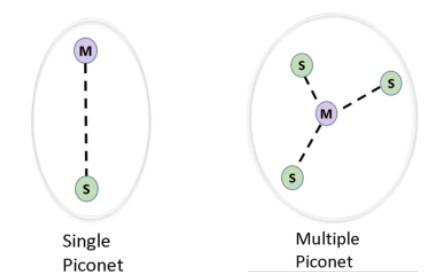
\includegraphics{Piconet}\\
  
    
    The Bluetooth network is called a piconet. If it contains one master and one slave then its called a single piconet. Similarly, if it contains one master and multiple slaves are called multiple piconets.
    

    The Master is the one that initiates the communication with other devices and it dictates when a slave device may transmit.
    
    Direct Slave to Slave communication is not possible.

    Maximum 7 active slaves can be present in multiple piconets, in other words, only 8 maximum devices including the master can communicate at any one time in a piconet.

    \section*{Scatternet}
    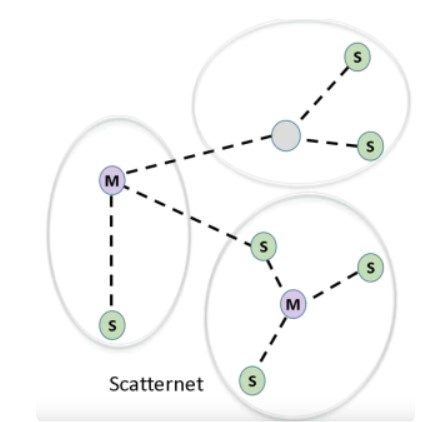
\includegraphics{Scatternet}\\
   
    Its a Combination of multiple piconets.

    Here Master of one piconet can be a slave in another piconet. This node can receive a message from a master in one piconet and deliver the message to its slave into the other piconet.

    Therefore, this type of node is referred to as a bridge node. Above all, a station cannot be master in two piconets.
    
    \section*{Architecture of a Bluetooth IoT Application}
    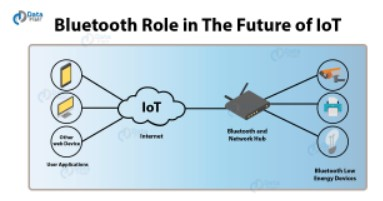
\includegraphics{IOT Architecture}\\

    Firstly, we must first dive into the Bluetooth “stack” to understand why recent shifts in Bluetooth standards are significant for IoT applications The evolution of Bluetooth from a replacement for RS-232 data cables to a powerful and massive IoT connectivity solution is a story of adding new layers to the stack. The newest Bluetooth specification for IoT—Bluetooth mesh—must be engineered upon either the BLE 4.xx or 5.xx stack—an extension of the Bluetooth Core (“classic”) specification. The emerging Bluetooth mesh stack, therefore, comprises three-stack layers: Core, then BLE, and mesh on top.

    \section*{Bluetooth Topologies: Pair, Broadcast, Mesh}

    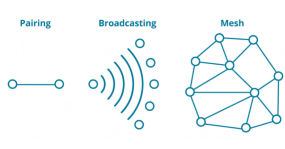
\includegraphics{BluetoothMesh}\\
    \begin{itemize}
        \item \textbf {Pair:} Bluetooth as a means of pairing two devices
For Example, a computer paired with a wireless mouse 
        \item \textbf {Broadcasting:} Bluetooth as a means of having one device broadcast information to many devices or vice versa
For Example: Playing music on smart speakers and simultaneously casting photos to a projector—both using a single iPhone
        \item \textbf {Mesh:} Bluetooth as a way of connecting many devices to many others as if in a spider’s web
For Example: Connecting 1,278 overhead lights in a warehouse to each other to dim and brighten lights automatically based upon activity and personal preferences.
    \end{itemize}

    \section*{Bluetooth Protocol Types}

    The main function of the Bluetooth is a Bluetooth protocol stack in architecture of bluetooth . In other words, It defines and provides different types of layers and functionalities. Bluetooth can run the different applications over different protocol stacks, but, each one of these protocol stacks uses the same Bluetooth link and physical layers.

    The below diagram shows a complete Bluetooth protocol stack. It shows the relationship between the protocols that use the services of other protocols when there is a payload to be transferred in the air. Anyhow, the protocols have many other relationships between the other protocols – for example, some protocols (L2CAP, TCS Binary) use the LMP to control the link manager.

    The complete protocol stack architecture of Bluetooth is made up of both Bluetooth specific protocols like object exchange protocols (OBEX) and user datagram protocol (UDP).

    The main principle is to minimize the reuse of current protocols for different purposes at higher layers as if re-inventing circle once again. The protocol re-use is helpful for the legacy applications to work with the Bluetooth technology to measure the smooth operations and interoperability of applications. Hence, many applications are being developed to take immediate advantage of the software and hardware.

    \textbf{    Protocol image}
 \section*{Bluetooth Protocols :} 
    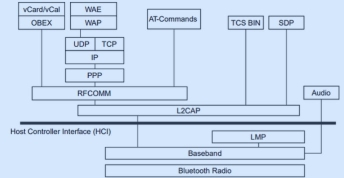
\includegraphics{protocols}\\
   \begin{align}
       
    \begin{tabular}{ | m{6em} | m{5cm} | } 
    \hline
    \textbf Protocol Layers & Protocol in the stacks\\ 
    \hline
    Bluetooth Core Protocol & Baseband, LMP, L2CAP, SDP \\ 
    \hline
    Cable Replacement Protocol & RFCOMM\\ 
    \hline
    Telephony Control Protocol & TCS Binary, AT- commands\\
    \hline
    Adopted Protocols & PPP, OBEX, UDP/TCP/IP, WAP, Vcard, Vcall, IrMC, WAE\\
    \hline

  \hline
\end{tabular}
  \end{align}

\section*{Advantages of Bluetooth Protocols} 
    \begin{itemize}
        \item Bluetooth offers economic wireless solutions (both data & voice) but, for short distances
        \item On the other hand, Mobile and stationary environment use Bluetooth protocol.
        \item There is no setup file to install the Bluetooth, in other words, it is an inbuilt device.
        \item Above all, They are up-gradable
    \end{itemize}

    \section*{Characteristics of Bluetooth Protocols} 
    \begin{itemize}
        \item In short, Up to eight devices including the master can communicate in the Piconet by using Bluetooth.
        \item Bluetooth signals are Omnidirectional as a result devices don’t point at each other.
        \item Governments regulated worldwide because it is possible to utilize the same standard.
        \item In short , Signals can transmit through walls and briefcases.
    \end{itemize}
    
\section*{Layers of Architecture of Bluetooth :} 
    \begin{center}
    \begin{tabular}{ | m{6em} | m{5cm} | } 
    \hline
    \textbf Host Controller Interface & A command interface for the controller and for the link manager, which allows access to the hardware status and control registers.\\ 
    \hline
    Logical Link Control and Adaptation Protocol & It is also known as the heart of the Bluetooth protocol stack. It allows the communication between the upper and lower layers of the Bluetooth protocol stack. \\ 
    \hline
    Radio (RF) layer & It performs modulation/demodulation of the data into RF signals\\ 
    \hline
    Baseband Link layer & In short, it performs the connection establishment within a piconet.\\
    \hline
    SDP layer & It is short for Service Discovery Protocol. It allows for discovering the services available on another Bluetooth enabled device.\\
    \hline
    WAP & It is short for Wireless Access Protocol. It is used for internet access.\\
    \hline
    TCS & It is short for Telephony Control Protocol. It provides a telephony service.\\
    \hline
    Application layer & 	In short , it enables the user to interact with the application.\\
    \hline

    \end{tabular}
    \end{center}

    \section*{Bluetooth Security } 
    
        
    Firstly, the security of any wireless technology is very important. With hackers gaining access to an ever-increasing number of systems, as a result,Bluetooth security is increasingly important.

    Bluetooth security must also address more specific Bluetooth related attacks that target known vulnerabilities in Bluetooth implementations and specifications. In other words, these may include attacks against improperly secured Bluetooth implementations which can provide attackers with unauthorized access.
 
    Many users may not believe there is
    an issue with Bluetooth security, but hackers may be able to gain access to information from phone lists to more sensitive information that others may hold on Bluetooth enabled phones and other devices.


    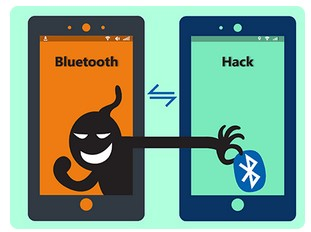
\includegraphics{security}
    \section* \textbf{Firstly, there are three basic means of providing Bluetooth security:}
    
    \begin{itemize}
        \item \textbf{Authentication: }  In this process, that is to say,the identity of the communicating devices is verified. But ,user authentication is not part of the main Bluetooth security elements of the specification.
        \item \textbf{Confidentiality: }  In Short, this process prevents the information from being eavesdropped by ensuring that only authorized devices can access and view the data. On the other hand, Mobile and stationary environment use Bluetooth protocol.
        \item \textbf{Authorization:  } This process prevents access by ensuring that a device is authorized to use a service before enabling it to do so. There is no setup file to install the Bluetooth, in other words, it is an inbuilt device.
    \end{itemize}

     \section*{Common Bluetooth security issues}
     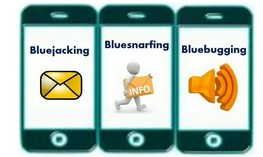
\includegraphics{issues}
    \begin{itemize}
        \item \textbf{Bluejacking:} In short, Sending spam messages to discoverable Bluetooth enabled devices. However, this form of hacking is harmless. In short, the best way to defend against it is to keep Bluetooth settings to invisible or non-discoverable.
        \item \textbf{Bluesnarfing:} It is more serious than bluejacking because it can reveal private information on a smartphone and is capable of happening even when invisible/non-discoverable mode is enabled.
        \item \textbf{Bluebugging:} In short, it’s capable of accessing all the information such as photos, apps, contacts, etc. It’s more dangerous than bluejacking and bluesnarfing.
    \end{itemize}
    
    \section* {Common Bluetooth security issues:}

    In Conclusion, Some prevention tips for Bluetooth hacks are to set invisible mode. Therefore, makes it more difficult for hackers to gain access to your data. Lastly, stay awake from the open Wi-Fi networks in busy or untrusted locations, so that you can minimize the risk of falling victim to hackers.

  
    
\end{multicols}
\end{document}

